\documentclass[10pt,letterpaper]{article}
\usepackage[dvipsnames]{xcolor}
\usepackage{outlines}
\usepackage{amsmath}
\usepackage{tikz}
\usepackage{hyperref}
\usepackage{enumitem}
\usepackage{cancel}
\usepackage{subcaption}
\DeclareCaptionOptionNoValue{centering}{\centering} % Make sure everything is centered in subs
\captionsetup[sub]{centering}

\usepackage{multirow}
\usepackage{cancel}
\usepackage{float}

\usepackage{parskip}

\usepackage{slantsc,lmodern}

\usepackage{pgfplotstable,booktabs}
\usepackage{framed}
\definecolor{shadecolor}{rgb}{0.9,0.9,0.9}

\usepackage{gensymb}

\usepackage{paralist}

\usepackage[paper=a4paper,margin=1in]{geometry}

\usepackage{etoolbox}

\newcommand{\volume}{{\ooalign{\hfil$V$\hfil\cr\kern0.08em--\hfil\cr}}}

\makeatletter
\g@addto@macro\@floatboxreset\centering
\makeatother

\author{Thaddeus Hughes \\ hughes.thad@gmail.com \\ thaddeus-maximus.github.io}
\date{\today}
\title{Simple Model of a Rocker Pod}



\begin{document}
	\maketitle
	
	\begin{abstract}
		\begin{figure}[H]
			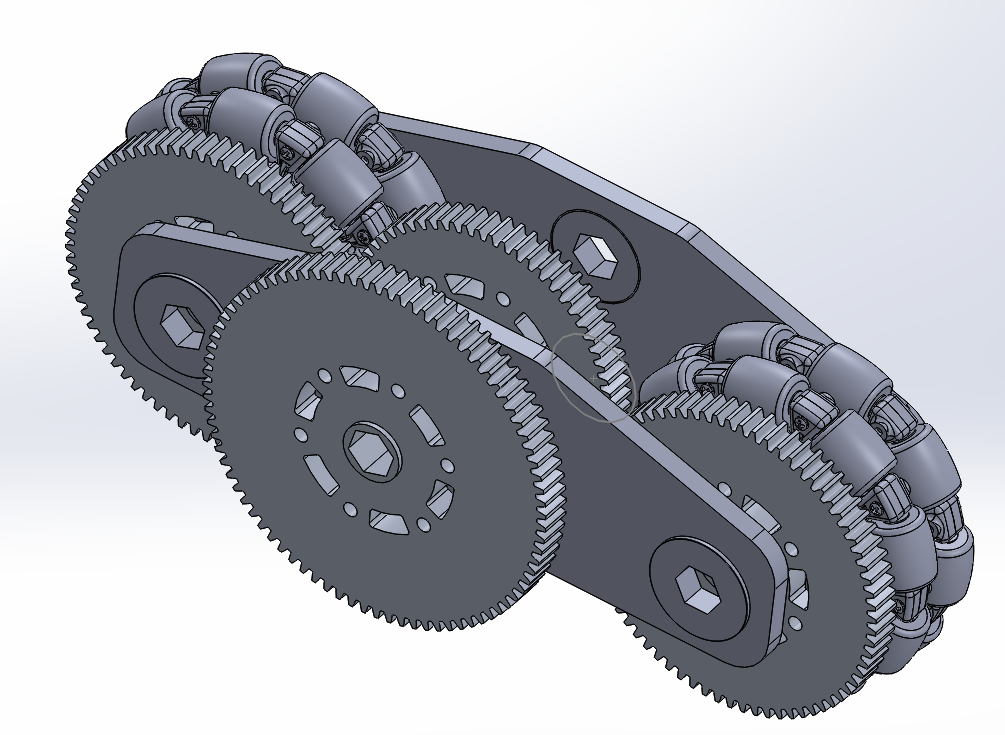
\includegraphics[width=0.7\textwidth]{drivetrain_slide_rocker.png}
			\caption{Rocker pod with omnis for use in a slide drive.}
		\end{figure}
		Rocker pods are very interesting mechanisms as they allow for a dynamic suspension system without the need for extra actuators, creating an amount of normal or contact force that is proportional to the driving torque. This is due to their tendency for the wheels to dig into the surface they contact, creating additional force beyond the input torque. This makes them excellent in slide drive applications, but they need to be properly designed in order to function properly. While \href{https://johnvneun.com/blog/2019/1/3/x019-prototype}{\color{red}\underline{the Robowranglers (FRC Team 148) pioneered their use in slide (H) drives}}, rocker pods also have applications beyond drivetrains such as \href{https://www.youtube.com/watch?v=q8VA5kmzAPk}{\color{red}\underline{in intake systems}}.
	\end{abstract}
	
	\section*{System Definition}
	
	Consider half of a rocker pod (the other half is simply the same principle, but in the reverse direction).	
	
\begin{figure}[H]
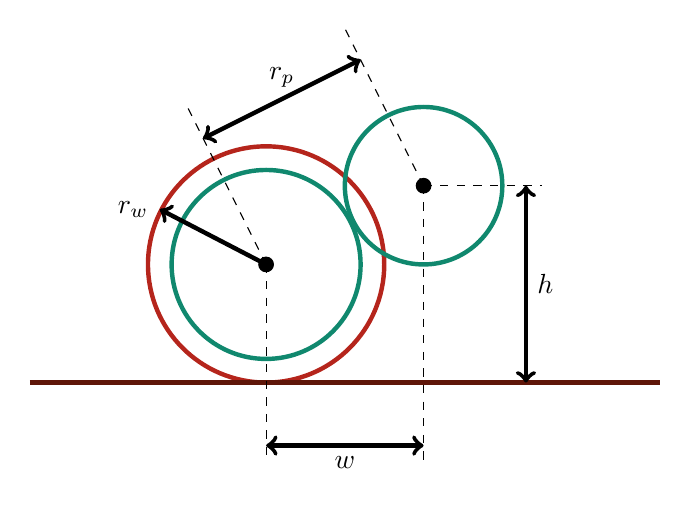
\begin{tikzpicture}
\draw[BrickRed,  ultra thick] (-2,-1) circle (1.5);
\draw[PineGreen, ultra thick] (0,0) circle(1);
\draw[PineGreen, ultra thick] (-2,-1) circle(1.2);
\draw[Sepia,     ultra thick] (-5,-2.5)--(3,-2.5);

\fill[black] ( 0, 0) circle (0.1);
\fill[black] (-2,-1) circle (0.1);

\draw[dashed] (-2,-1) -- (-3,1);
\draw[dashed] ( 0, 0) -- (-1,2);
\draw[<->, ultra thick] (-2.8, 0.6) -- (-0.8,1.6) node[pos=0.5,above]{$r_{p}$};
\draw[dashed] ( 0, 0) -- (1.5,0);
\draw[<->, ultra thick] (1.3,0)--(1.3,-2.5) node[pos=0.5, right]{$h$};

\draw[->, ultra thick] (-2,-1) -- (-3.35,-0.3) node[pos=1, left]{$r_{w}$};

\draw[dashed] (-2,-1) -- (-2,-3.5);
\draw[dashed] (0,0)   -- (0, -3.5);
\draw[<->, ultra thick] (-2, -3.3) -- (0, -3.3) node[pos=0.5, below]{$w$};

\end{tikzpicture}
\caption{Dimensions critical to rocker pod functionality. Gears in green, wheel in red.}
\end{figure}

By pythagorean theorem,

\begin{align}
	w = \sqrt{r_{p}^2 - (h - r_{w})^2}
\end{align}

\begin{figure}[H]
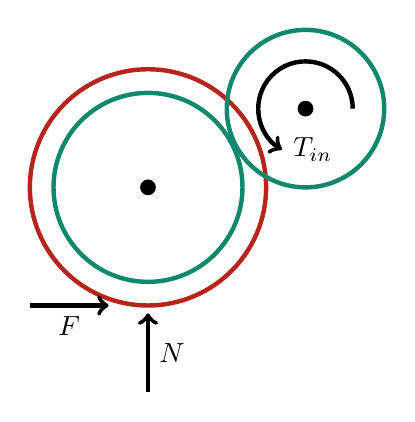
\begin{tikzpicture}
\draw[BrickRed,  ultra thick] (-2,-1) circle (1.5);
\draw[PineGreen, ultra thick] (0,0) circle(1);
\draw[PineGreen, ultra thick] (-2,-1) circle(1.2);

\fill[black] ( 0, 0) circle (0.1);
\fill[black] (-2,-1) circle (0.1);

\draw[->, ultra thick] (-2,-3.6)--(-2,-2.6) node [pos=0.5,right]{$N$};
\draw[->, ultra thick] (-3.5,-2.5)--(-2.5,-2.5) node [pos=0.5,below]{$F$};

\draw[->, ultra thick] (0.6,0) arc (0:240:0.6) node [pos=1,right]{$T_{in}$};

\end{tikzpicture}
\qquad
\qquad
\qquad
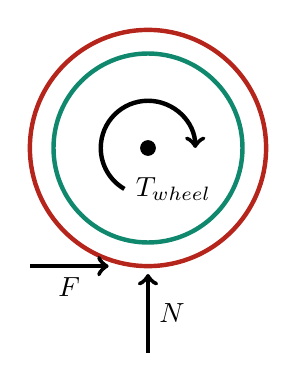
\begin{tikzpicture}
\draw[BrickRed,  ultra thick] (-2,-1) circle (1.5);
\draw[PineGreen, ultra thick] (-2,-1) circle(1.2);

\fill[black] (-2,-1) circle (0.1);

\draw[->, ultra thick] (-2,-3.6)--(-2,-2.6) node [pos=0.5,right]{$N$};
\draw[->, ultra thick] (-3.5,-2.5)--(-2.5,-2.5) node [pos=0.5,below]{$F$};

\draw[<-, ultra thick] (-1.4,-1) arc (0:240:0.6) node [pos=1,right]{$T_{wheel}$};

\end{tikzpicture}
\caption{Left: free-body diagram of a half rocker pod. Right: free-body diagram of its wheel.}
\end{figure}

\section*{Physics Principles}

Applying conservation of angular momentum to the rocker pod yields

\begin{align}
	\cancelto{\mbox{0 (lightweight system)}}{\frac{d}{dt} L_{sys}} = \sum_{about\ pivot} \vec{r} \times \vec{F} + \cancelto{\mbox{0 (no mass transfer)}}{\sum_{+in} \dot{m} [...]} \nonumber \\
	h F - w N + T_{in} = 0 .
\end{align}

Applying conservation of angular momentum to the wheel yields

\begin{align}
	\cancelto{\mbox{0 (lightweight system)}}{\frac{d}{dt} L_{sys}} = \sum_{about\ axle} \vec{r} \times \vec{F} + \cancelto{\mbox{0 (no mass transfer)}}{\sum_{+in} \dot{m} [...]} \nonumber \\
	r_{w} F - T_{wheel} = 0 .
\end{align}

The wheel torque is related to the input torque by module gear ratio $G$.

\begin{align}
	T_{wheel} = G \ T_{in}
\end{align}

A negative $G$ could be input to simulate a module that did not reverse the input and output directions.

The wheel's force should be friction-limited. We'll use a simple static friction model with $\mu$ as the coefficient of friction.

\begin{align}
	F \leq \mu N	
\end{align}

\section*{Solution}

The various constraints can be solved, yielding

\begin{align}
	F &= \frac{G}{r_{w}} T_{in} \\
	N &= \frac{1 + G \frac{h}{r_{w}}}{\sqrt{r_{p}^2 - (h - r_{w})^2}} T_{in}
\end{align}

The ratio of propulsive force to normal force can also be solved for, which would be the effective frictional coefficient of the module.

\begin{align}
	F/N = \mu_{effective} = \frac{\frac{G}{r_{wheel}}}{ 1 + G \frac{h}{r_{wheel}} } \sqrt{r_{p}^2 - (h - r_{w})^2}
\end{align}

This ratio should be kept beneath the coefficient of friction, otherwise the module would slip. It also should not be kept too low, otherwise the normal force will be large even at small amounts of propulsion.

My \href{https://thaddeus-maximus.github.io/swissarmyengineer/rockerpod}{\color{red}\underline{Swiss Army Engineer Tool}} contains a rocker pod analyzer that can be used to perform these calculations.
	
\end{document}